\documentclass[10pt]{mypackage}

% sans serif font:
%\usepackage{cmbright,sfmath,bbold}
%\renewcommand{\mathcal}{\mathtt}

%Euler:
\usepackage{newpxtext,eulerpx,eucal,eufrak}
\renewcommand*{\mathbb}[1]{\varmathbb{#1}}
\renewcommand*{\hbar}{\hslash}

%\usepackage{homework}

\pagestyle{fancy} %better headers
\fancyhf{}
\rhead{Avinash Iyer}
\lhead{Mathematical Methods II Notes}

\setcounter{secnumdepth}{0}

\begin{document}
\RaggedRight
\section{Complex Analysis}%
\subsection{Analyticity and Path-Independence in the Complex Plane}%
\subsubsection{Baby's First Complex Function Theory}%
We are interested in functions of the form $f(z)$, where $z = x+iy$ is some complex number. Note that this is specifically different from a function $g\colon \R^2\rightarrow \Omega$ for some domain $\Omega$; in the latter case, we have independent variables $x$ and $y$, while in the former case, we must express $z = x+iy$.\newline

Now, consider a contour integral
\begin{align*}
  \oint_{C}^{} w(z)\:dz &= \oint_{C}w(z)\:\left(dx + idy\right)\\
                        &= \oint_{C}^{} w(z)\:dx + i\oint_{C}w(z)\:dy.
                        \intertext{Taking $A_x = w(z)$ and $A_y = iw(z)$, we have}
                        &= \oint_{C}^{} \mathbf{A}\cdot\:d\vec{\ell}.
                  \intertext{We want to know if this is equal to, by Green's Theorem,}
                        &= \int_{S}^{} \left(\nabla\times \mathbf{A}\right)\:d\mathbf{a},
\end{align*}
and when this integral is zero. Note that $\left(\nabla\times \mathbf{A}\right)\cdot \hat{n} = 0$, so $\pd{A_y}{x} - \pd{A_x}{y} = 0$.\newline

Note that we can take
\begin{align*}
  w(z) &= u(x,y) + iv(x,y),
\end{align*}
where $z = x + iy$.\newline

After a lot of tedious derivation, we get the Cauchy--Riemann equations.
\begin{theorem}[Cauchy--Riemann Equations]
  \begin{align*}
    \pd{u}{x} &= \pd{v}{y}\\
    \pd{v}{x} &= -\pd{u}{y}.
  \end{align*}
\end{theorem}
Furthermore, the Cauchy--Riemann equations guarantee that $w$ is analytic,\footnote{Equal to its Taylor series, also holomorphic.} which leads to Cauchy's theorem.
\begin{theorem}[Cauchy's Theorem]
  If $C$ is a simple closed curve in a simply connected region, then $w$ is analytic if and only if
  \begin{align*}
    \oint_{C}^{} w(z)\:dz &= 0.\label{thm:cauchy_integral_thm}\tag{\textdagger}
  \end{align*}
\end{theorem}
\begin{fact}
The function $w(z)$ is analytic inside the simply connected region $R$ if any of these hold:
\begin{itemize}
  \item $w$ satisfies the Cauchy--Riemann equations;
  \item $w'(z)$ is unique and exists;
  \item $\pd{w}{\overline{z}} = 0$.
  \item $w$ can be expanded in a Taylor series convergent on some open neighborhood of $z$: $w(z) = \sum_{n\geq 0}c_n\left(z-a\right)^n$;\footnote{This is the real definition of analytic.}
  \item $w(z)$ is path-independent everywhere in $R$: $\oint_{C}w(z)\:dz = 0$.
\end{itemize}
\end{fact}
\begin{example}
  Considering $w(z) = z$, we have $u=x$ and $v=y$, so it satisfies the Cauchy--Riemann equations. However, neither $\re\left(z\right)$ nor $\im\left(z\right)$ are analytic, and neither is $\overline{z} = x-iy$.
\end{example}
\begin{remark}
Whenever we say ``analytic at $p$,'' we mean ``analytic in a neighborhood of $p$.''
\end{remark}
Note that since $\C$ is a non-compact locally compact Hausdorff space, we may carry out a one-point compactification of $\C$, by adjoining a point $\set{\infty}$, $\C^{\ast} = \C\cup \set{\infty}$. This compactified $\C^{\ast}$ is often represented as a unit sphere with the north pole, determined by $\left(0,0,1\right)$, is the point at infinity. The correspondence between $\C^{\ast}\setminus\set{\infty}$ and $\C$ is evaluated via stereographic projection.\newline

We define $\frac{z}{\infty} = 0$ and $\frac{z}{0} = \infty$ for any $z\neq 0,\infty$. The correspondence between $z = x + iy$ in the plane to $Z$ on the Riemann sphere with $\R^3$ coordinates $\left(\xi_1,\xi_2,\xi_3\right)$ is
\begin{align*}
  \xi_1 &= \frac{2\re(z)}{\left\vert z \right\vert^2 + 1}\\
  \xi_2 &= \frac{2\im\left(z\right)}{\left\vert z \right\vert^2 + 1}\\
  \xi_3 &= \frac{\left\vert z \right\vert^2 - 1}{\left\vert z \right\vert^2 + 1}.
\end{align*}
Inverting, we may find
\begin{align*}
  x &= \frac{\xi_1}{1-\xi_3}\\
  y &= \frac{\xi_2}{1-\xi_3},
\end{align*}
and with polar coordinates,
\begin{align*}
  z &= \cot\left(\theta/2\right)e^{i\phi}.
\end{align*}

\begin{center}
  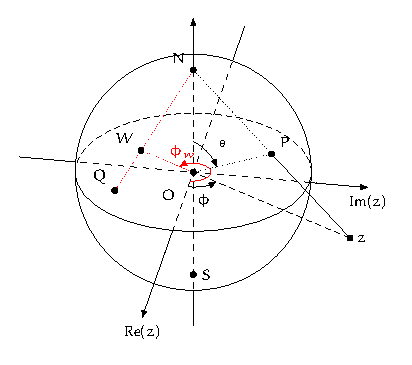
\includegraphics[width=7cm]{images/riemann_sphere.pdf}
\end{center}
To determine analyticity at $\infty$, we set $\zeta = \frac{1}{z}$, and analyze the analyticity of $\tilde{w}\left(\zeta\right) = w\left(1/z\right)$ at $0$.
\subsubsection{Cauchy's Integral Formula}%
Consider the function $w(z) = c/z$, integrated around a circle of radius $R$. Then, writing $z = Re^{i\varphi}$, we get
\begin{align*}
  \oint_{\Gamma}w(z)\:dz &= C\int_{0}^{2\pi} \frac{e^{-i\varphi}}{R}\underbrace{iRe^{i\varphi}\:d\varphi}_{dz}\\
                         &= ic\int_{0}^{2\pi} \:d\varphi\\
                         &= 2\pi i c.
\end{align*}
If our contour $C$ runs around our singularity at $z = 0$ a total of $n$ times, then we pick up a factor of $n$.\newline

Now, when we consider
\begin{align*}
  I &= \oint_{C}\frac{dz}{z^n},
\end{align*}
this integral actually yields $0$ for any $n\neq 1$, despite the fact that $0$ is a singularity for $f(z) = \frac{1}{z^n}$. This $0$ is not a reflection of \eqref{thm:cauchy_integral_thm}, but of the fact that
\begin{align*}
  z^{-n} &= \frac{d}{dz}\left(\frac{z^{-n+1}}{n+1}\right),
\end{align*}
meaning that $z^{-n}$ is an exact differential, so integrating along a closed curve yields zero change. However, $\frac{1}{z} = \diff{}{z}\left(\ln z\right)$ may be an exact differential, but for complex $z$, $\ln z = \ln\left\vert z \right\vert + i\arg(z) = \ln r + i\varphi$. This yields
\begin{align*}
  \oint_{C} \frac{c}{z}dz &= c\oint_{C} d\left(\ln z\right)\\
                          &= c\left(i\left(\varphi + 2\pi\right) - \varphi\right)\\
                          &= 2\pi i c.
\end{align*}
Ultimately, what this shows is that when we integrate any analytic function $f\left(\zeta\right)$ along a closed contour with a singularity at $z$, only the coefficient on $\frac{1}{\zeta -z}$ will remain. This coefficient is known as the residue at $0$.
\begin{theorem}[Cauchy's Integral Formula]
  If $w$ is analytic in a simply connected region and $C$ is a closed contour winding once around a point $z$ in the region, then
  \begin{align*}
    w(z) &= \frac{1}{2\pi i} \oint_{C}\frac{w\left(\zeta\right)}{\zeta - z}\:d\zeta.
  \end{align*}
\end{theorem}
Furthermore, this shows that any once-differentiable function is infinitely differentiable, as by differentiating under the integral sign, we get
\begin{align*}
  \diff{^nw}{z^n} &= \frac{n!}{2\pi i} \oint_{C} \frac{w\left(\zeta\right)}{\left(\zeta - z\right)^{n+1}}\: d\zeta.
\end{align*}
\begin{example}[Deriving Liouville's Theorem]
  Consider a circle $C$ centered at radius $r$ centered at at $z$, $\zeta - z = Re^{i\varphi}$. We take $d\zeta = iRe^{i\varphi}\:d\varphi$, and taking derivatives, we have
  \begin{align*}
    w'(z) &= \frac{1}{2\pi R} \int_{0}^{2\pi} w\left(z + Re^{i\varphi}\right)e^{-i\varphi}\:d\varphi.
  \end{align*}
  If $w$ is bounded --- i.e., $\left\vert w(z) \right\vert \leq M$ for all $z$ in a given region --- then
  \begin{align*}
    \left\vert w'(z) \right\vert &= \left\vert \frac{1}{2\pi R} \int_{0}^{2\pi} w\left(z + Re^{i\varphi}\right)e^{-i\varphi}\:d\varphi \right\vert\\
                                 &\leq \frac{1}{2\pi R} \int_{0}^{2\pi} \left\vert w\left(z + Re^{i\varphi}\right) \right\vert\:d\varphi\\
                                 &\leq \frac{M}{R}
  \end{align*}
  for all $R$ within the analytic region.\newline

  In the case where $w$ is entire (i.e., analytic on $\C$), then this inequality holds for all $R\rightarrow\infty$. Thus, $\left\vert w'(z) \right\vert = 0$ for all $z$, meaning that $w$ is constant.\newline

  This is known as Liouville's theorem --- every bounded entire function is constant. This can be used to prove the fundamental theorem of algebra.\newline

  What Liouville's theorem tells us is that any nontrivial behavior will emerge from a function's singularities.
\end{example}
\subsection{Singularities and Branches}%
To understand nontrivial behavior on the complex plane, we need to understand singularities. This will require us to develop understanding of Laurent series.
\subsubsection{Taylor Series}%
We want to integrate $w(z)$ around some point $a$ in an analytic region of $w(z)$. This yields the form
\begin{align*}
  w(z) &= \frac{1}{2\pi i} \oint_{C}^{} \frac{w\left(\zeta\right)}{\zeta - z}\:d\zeta\\
       &= \frac{1}{2\pi i} \oint_{C} \frac{w\left(\zeta\right)}{\left(\zeta - a\right)-\left(z-a\right)}\:d\zeta\\
       &= \frac{1}{2\pi i} \oint_{C} \frac{w\left(\zeta\right)}{\left(\zeta - a\right)\left(1 - \frac{z-a}{\zeta - a}\right)}\:d\zeta.\label{step:geometric_expansion}\tag{\textdaggerdbl}
       \intertext{Since $\zeta$ is on the contour and $z$ is in the contour, $\left\vert \frac{z-a}{\zeta - a} \right\vert < 1$, we may expand as a geometric series. Thus, we get}
       &= \frac{1}{2\pi i} \oint_{C} \frac{w\left(\zeta\right)}{\left(\zeta - a\right)}\left(\sum_{n=0}^{\infty}\left(\frac{z-a}{\zeta - a}\right)^{n}\right)\:d\zeta.
       \intertext{Since the series is uniformly convergent, we are allowed to exchange sum and integral, yielding}
       &= \sum_{n=0}^{\infty}\underbrace{\left(\frac{1}{2\pi i}\oint_{C}\frac{w\left(\zeta\right)}{\left(\zeta - a\right)^{n+1}}\:d\zeta\right)}_{=c_n} \left(z-a\right)^n\\
       &= \sum_{n=0}^{\infty}c_n\left(z-a\right)^n,
       \intertext{where}
  c_n &= \frac{1}{n!} \left.\diff{^nw}{z^n}\right|_{z=a}.
\end{align*}
If our Taylor series reduces to a known series on the real axis, we find this very desirable. We say this is a type of analytic continuation from the real axis to the complex plane. For example,
\begin{align*}
  e^z &= \sum_{k=0}^{\infty}\frac{z^k}{k!}
\end{align*}
is an analytic continuation of $e^x$.\newline

However, more interestingly,
\begin{align*}
  \zeta\left(s\right) &= \sum_{k=1}^{\infty}\frac{1}{k^s}
\end{align*}
converges for all $s > 1$. However, we have also shown that
\begin{align*}
  \zeta\left(s\right) &= \frac{1}{\Gamma(s)}\int_{0}^{\infty} \frac{x^{s-1}}{e^{x}-1}\:dx
\end{align*}
converges for complex $s$ for all real part greater than $1$. Since values of this integral agree with the series representation of $\zeta(s)$ on real axis, we have that this is an analytic continuation of $\zeta(s)$ to the subset of $\C$ defined by $\re(s) > 1$.
\subsubsection{Laurent Series}%
Now, what happens if, at \eqref{step:geometric_expansion}, we have $\left\vert \frac{z-a}{\zeta - a} \right\vert > 1$. The series as constructed would not converge, but what if we have a series that converges everywhere \textit{outside} $C$? This would entail an expansion in reciprocal integer powers of $z-a$. This yields
\begin{align*}
  w(z) &= -\frac{1}{2\pi i} \oint_{C}\frac{w\left(\zeta\right)}{\left(z-a\right)\left(1-\frac{\zeta - a}{z-a}\right)}\:d\zeta\\
       &= -\frac{1}{2\pi i} \oint_{C} \frac{w\left(\zeta\right)}{z-a}\left(\sum_{n=0}^{\infty}\left(\frac{\zeta - a}{z-a}\right)^n\right)\:d\zeta\\
       &= -\sum_{n=0}^{\infty}\left(\frac{1}{2\pi i}\oint_{C}w\left(\zeta - a\right)^n\:d\zeta\right)\frac{1}{\left(z-a\right)^{n+1}}\\
       &= \sum_{n=1}^{\infty}\underbrace{\left(-\frac{1}{2\pi i}\oint_{C}w\left(\zeta - a\right)^{n-1}\:d\zeta\right)}_{=c_{-n}}\frac{1}{\left(z-a\right)^{n}}\\
       &= \sum_{n=1}^{\infty}\frac{c_{-n}}{\left(z-a\right)^n}
\end{align*}
Note that this series has a singularity at $z = a$, but since our series is only defined outside a particular region, that doesn't matter. We call a series in reciprocal powers a Laurent series.
\end{document}
